%\documentclass{article}
\documentclass[5pt]{article}

\usepackage{fancyhdr}
\usepackage{extramarks}
\usepackage{amsmath}
\usepackage{amsthm}
\usepackage{amsfonts}
\usepackage{amssymb}
\usepackage{tikz}
\usepackage[plain]{algorithm}
\usepackage{algpseudocode}
\usepackage{enumitem}
\usepackage{mathtools}
\usepackage{hyperref}
\usepackage[all]{hypcap} % fixes the wrong figure jumping issue

%% matlab stuff
\usepackage{listings}
\usepackage{color} %red, green, blue, yellow, cyan, magenta, black, white
\definecolor{mygreen}{RGB}{28,172,0} % color values Red, Green, Blue
\definecolor{mylilas}{RGB}{170,55,241}



\usetikzlibrary{automata,positioning}

%
% Basic Document Settings
%

\topmargin=-0.45in
\evensidemargin=0in
\oddsidemargin=0in
\textwidth=6.5in
\textheight=9.0in
\headsep=0.25in

\linespread{1.1}

\pagestyle{fancy}
\lhead{\hmwkAuthorName}
\chead{\hmwkClass\ (\hmwkClassInstructor): \hmwkTitle}
%\rhead{\firstxmark}
%\lfoot{\lastxmark}
%\cfoot{\thepage}

\renewcommand\headrulewidth{0.4pt}
\renewcommand\footrulewidth{0.4pt}


\setlength\parindent{0pt}

%
% Create Problem Sections
%

\newcommand{\enterProblemHeader}[1]{
    \nobreak\extramarks{}{Problem \arabic{#1} continued on next page\ldots}\nobreak{}
    \nobreak\extramarks{Problem \arabic{#1} (continued)}{Problem \arabic{#1} continued on next page\ldots}\nobreak{}
}

\newcommand{\exitProblemHeader}[1]{
    \nobreak\extramarks{Problem \arabic{#1} (continued)}{Problem \arabic{#1} continued on next page\ldots}\nobreak{}
    \stepcounter{#1}
    \nobreak\extramarks{Problem \arabic{#1}}{}\nobreak{}
}

\setcounter{secnumdepth}{0}
\newcounter{partCounter}
\newcounter{homeworkProblemCounter}
\setcounter{homeworkProblemCounter}{1}
\nobreak\extramarks{Problem \arabic{homeworkProblemCounter}}{}\nobreak{}

%
% Homework Problem Environment
%
% This environment takes an optional argument. When given, it will adjust the
% problem counter. This is useful for when the problems given for your
% assignment aren't sequential. See the last 3 problems of this template for an
% example.
%
%\newenvironment{homeworkProblem}[1][-1]{
%    \ifnum#1>0
%        \setcounter{homeworkProblemCounter}{#1}
%    \fi
    %\section{Problem \arabic{homeworkProblemCounter}}
%    \setcounter{partCounter}{1}
    %\enterProblemHeader{homeworkProblemCounter}
%}{
    %\exitProblemHeader{homeworkProblemCounter}
%}

%
% Homework Details
%   - Title
%   - Due date
%   - Class
%   - Section/Time
%   - Instructor
%   - Author
%

\newcommand{\hmwkTitle}{Homework\ \#1}
\newcommand{\hmwkDueDate}{April 28, 2016}
\newcommand{\hmwkClass}{Stats 202C}
\newcommand{\hmwkClassInstructor}{Professor S.C. Zhu}
\newcommand{\hmwkAuthorName}{Eric Chuu}
\newcommand{\N}{\mathbb{N}}
\newcommand{\Z}{\mathbb{Z}}
\newcommand{\R}{\mathbb{R}}
\newcommand{\Q}{\mathbb{Q}}
\newcommand{\lnorm}{\left\Vert\left}
\newcommand{\rnorm}{\right\Vert\right}
%
% Title Page
%

\title{
    %\vspace{2in}
    \textmd{\textbf{\hmwkClass:\ \hmwkTitle}}\\
    \vspace{0.1in}\large{\textit{\hmwkClassInstructor\ \hmwkClassTime} \\ Assignment: 1-4}
    \author{\textbf{\hmwkAuthorName} \\ UID: 604406828}
}

%\author{\textbf{\hmwkAuthorName} \\ UID: 604406828}

\renewcommand{\part}[1]{\textbf{\large Part \Alph{partCounter}}\stepcounter{partCounter}\\}

%
% Various Helper Commands
%

% Useful for algorithms
\newcommand{\alg}[1]{\textsc{\bfseries \footnotesize #1}}

% For derivatives
\newcommand{\deriv}[1]{\frac{\mathrm{d}}{\mathrm{d}x} (#1)}

% For partial derivatives
\newcommand{\pderiv}[2]{\frac{\partial}{\partial #1} (#2)}

% Integral dx
\newcommand{\dx}{\mathrm{d}x}

% Alias for the Solution section header
\newcommand{\solution}{\textbf{\large Solution}}

% Probability commands: Expectation, Variance, Covariance, Bias
\newcommand{\E}{\mathrm{E}}
\newcommand{\Var}{\mathrm{Var}}
\newcommand{\Cov}{\mathrm{Cov}}
\newcommand{\Bias}{\mathrm{Bias}}
\newcommand{\isum}{\sum_{i=1}^n}
\newcommand{\jsum}{\sum_{j=1}^n}
\newcommand{\infint}{\int_{-\infty}^{\infty}}
\newcommand{\bin}{\mathrm{Bin}}
\newcommand{\geom}{\mathrm{Geom}}
\newcommand{\poi}{\mathrm{Poi}}
\newcommand{\expo}{\mathrm{Exp}}
\newcommand{\mgfx}{M_X(t)}
\newcommand{\mgfy}{M_Y(t)}
\newcommand{\pr}{\mathbf{Pr}}
\newcommand{\xvec}{\mathbf{x}}
\newcommand{\yvec}{\mathbf{y}}
\newcommand{\xbar}{\bar{X}}
\newcommand{\ybar}{\bar{Y}}
\newcommand{\samplechi}{\frac{(n-1)s^2}{\sigma^2}}

\newcommand{\vertii}[1]{{\left\vert\kern-0.25ex\left\vert #1 
    \right\vert\kern-0.25ex\right\vert}}

\newcommand{\verti}[1]{{\left\vert #1 
    \right\vert}}   

\newcommand\floor[1]{\lfloor#1\rfloor}
\newcommand\ceil[1]{\lceil#1\rceil}

%\[
%  d(x,y) = \left\{\def\arraystretch{1.2}%
%  \begin{array}{@{}c@{\quad}l@{}}
%    {0  & \text{if $x = y$}\\
%    {1 & \text{for $x < y$}\\
%    {2 & \text{for $x > y$}\\
%  \end{array}\right.
%\]




\begin{document}

\lstset{language=Matlab,%
    %basicstyle=\color{red},
    breaklines=true,%
    morekeywords={matlab2tikz},
    keywordstyle=\color{blue},%
    morekeywords=[2]{1}, keywordstyle=[2]{\color{black}},
    identifierstyle=\color{black},%
    stringstyle=\color{mylilas},
    commentstyle=\color{mygreen},%
    showstringspaces=false,%without this there will be a symbol in the places where there is a space
    numbers=left,%
    numberstyle={\tiny \color{black}},% size of the numbers
    numbersep=9pt, % this defines how far the numbers are from the text
    emph=[1]{for,end,break},emphstyle=[1]\color{red}, %some words to emphasise
    %emph=[2]{word1,word2}, emphstyle=[2]{style},    
}




\maketitle


\section{Problem 1} \\

\textbf{(1)}  The period of a state $i$ is given by
\begin{align}
	& d_i = \mathrm{gcd} \{ n \geq 1 : K_{ii}^{n} > 0 \}
\end{align}
We also know that a state $i$ is aperiodic if $d_i = 1$. \\

For $K_0$, we draw the transition graph diagram and see that all states can be reached in finite time with nonzero probability, so it is irreducible. Since the Markov chain is irreducible, then all states have the same period. Thus, it suffices to find the period of any state. If we begin in state 1, we can return to state 1 in two steps by going to state 2 and then back to state 1. We can also return to state 1 in three steps by going to state 2 then state 3, then returning back to state 1 directly. Then, $d_1 = 1$, and state 1 is aperiodic, and we conclude that $K_0$ is aperiodic. \\

For $K_1$, we can see from the transition graph diagram, $d_i = 1$ for $i = 1, \ldots, 5$, so $K_1$ is aperiodic. We can see that $K_1$ is reducible by considering states 5 and 4. If we are in states 4 or 5, the probability of going into states 1, 2, or 3 is 0. \\

For $K_2$, we draw the transition graph diagram and see that all states can be reached in finite time with nonzero probability, so it is irreducible. For each state, we can see that $d_i = 2$ for $i = 1, \ldots, 5$, so $K_2$ is periodic. \\

\textbf{(2)} The eigenvalues and left eigen-vectors for each matrix are given below. \\


\textbf{(3)} For each matrix, there are (insert number here) invariant probabilities. \\


\textbf{(4)} The eigen-values for $K_0, K_0^{50}, K_{0}^{200}$ are plotted below. \\

\begin{figure}[H]
\begin{center}
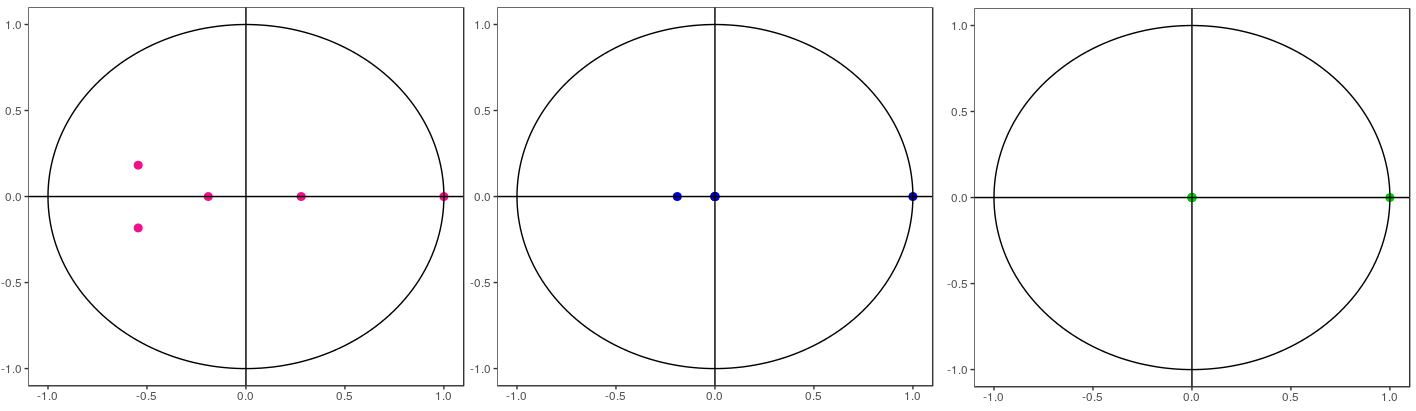
\includegraphics[width = 1 \columnwidth]{eigen_values}
\caption{Left: Eigenvalues for $K_0$. Center: Eigenvalues for $K_0^{50}$. Right: Eigenvalues for $K_0^{200}$}
\end{center}
\end{figure}


\textbf{(5)} We compute the matrix $K_0^{200}$, and we see that it becomes the ``ideal'' matrix, where each row is $\pi$.

\begin{align*}
K_0^{200} = 
	\begin{bmatrix}
		0.809 & 0.2512 & 0.3071 & 0.2389 & 0.1219 \\		
		0.809 & 0.2512 & 0.3071 & 0.2389 & 0.1219 \\	
		0.809 & 0.2512 & 0.3071 & 0.2389 & 0.1219 \\	
		0.809 & 0.2512 & 0.3071 & 0.2389 & 0.1219 \\	
		0.809 & 0.2512 & 0.3071 & 0.2389 & 0.1219
	\end{bmatrix}
\end{align*}

\hfill $\qed$

\pagebreak

\section{Problem 2}

\textbf{(1)} The plot of $d_{\mathrm{TV}}(n), d_{\mathrm{KL}}(n)$ for the first 200 steps is shown below.

\textbf{(2)} We calculate the contraction coefficient $K_0$ using
\begin{align}
	& C(K_0) = \max_{x, y} \vertii{K_0(x, \cdot) - K_0(y, \cdot)}_{\mathrm{TV}}
\end{align}

For two initial probbailities $\nu_1, \nu_2$,
\begin{align}
	& \vertii{\nu_1 \cdot K_0 - \nu_2 \cdot K_0}_{\mathrm{TV}} \leq C(K_0) \vertii{\nu_1 - \nu_2}_{\mathrm{TV}}
\end{align}

As $\vertii{\nu_1 - \nu_2}_{\mathrm{TV}} \leq 1$, if $C(K) < 1$, then the convergence rate can be upper bounded by

\begin{align}
	& A(n) = \vertii{\nu_1 \cdot K_0^n - \nu_{2} \cdot K_0^n}_{\mathrm{TV}} 
	\leq C^n(K_0) \vertii{\nu_1 - \nu_2}_{\mathrm{TV}} \leq C^n(K_0), \quad \forall \nu_1, \nu_2
\end{align}

The plot for the bound $C^n(K_0)$ over $n = 1, \ldots, 100$ is shown below.

\textbf{(3)} The Diaconis-Hanlon bound is given by
\begin{align}
	& B(n) = \vertii{\pi - \nu K_0^n}_{\mathrm{TV}} \leq \sqrt{\frac{1 -\pi(x_0)}{4 \pi (x_0)}} \lambda_{\mathrm{slem}}^n
\end{align}
where $x_0 = 1$ is the initial state and $\pi(x_0)$ is the target probability at $x_0 = 1$ and $\lambda_{\mathrm{slem}}^n$ is the second largest eigen-value modulus. The plot of the real convergence $d_{\mathrm{TV}}$ in comparison with $A(n), B(n)$ is given below. \\


We see that both converge to 0 very quickly, with KL-Divergence converging to 0 slightly faster. Bound $A(n)$, calculated using the contraction coefficient is shown in the turquoise curve below, while Bound $B(n)$, the Diaconis-Hanlon bound, is shown in the purple curve below. We can see that $B(n)$ provides a tighter bound on the convergence than does $A(n)$. \\

\begin{figure}[H]
\begin{center}
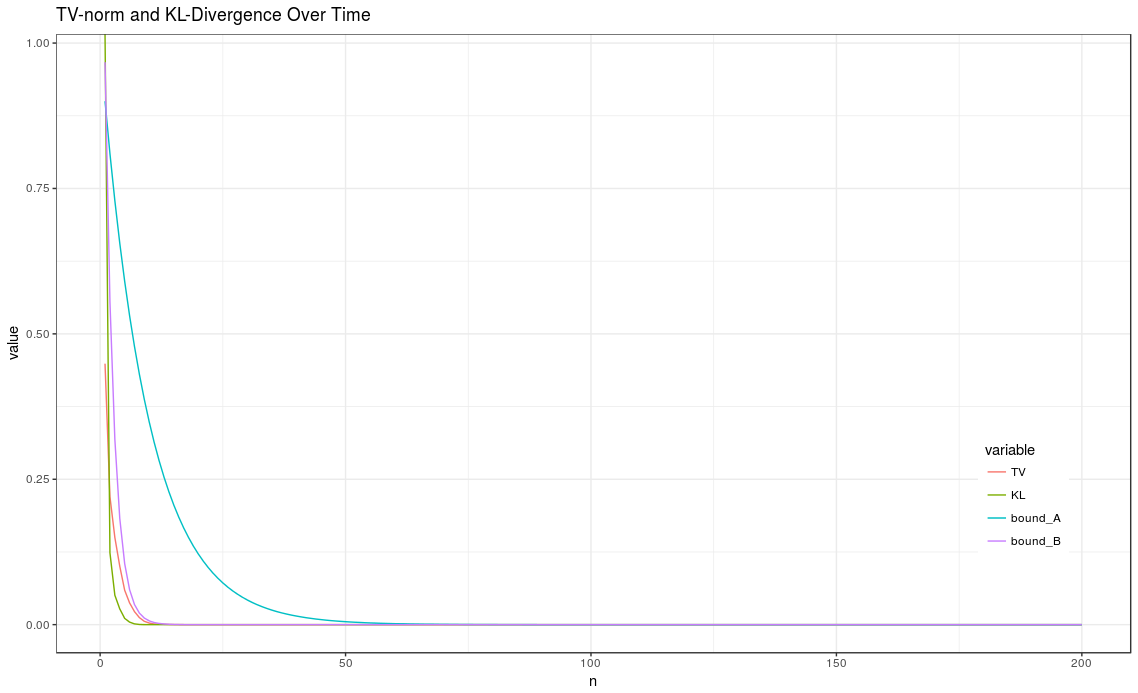
\includegraphics[width = 0.9\columnwidth]{q2_plot}
\caption{TV-norm and KL-Divergence for $n = 200$ steps. Bound A and Bound B refer to $A(n), B(n)$, respectively, both as calculated above.}
\end{center}
\end{figure}





\pagebreak

\section{Problem 3}
Show that the Kullback-Leibler divergence decreases monotonically,
\begin{align}
	& KL \left( \pi || \nu \right) - KL \left( \pi || \mu \right) = \E\left[
	KL \left( P \left( y, x \right) || Q\left( y, x \right) \right] \geq 0
\end{align}


\textbf{Solution} \\

\end{document}
